% section | subsection | subsubsection | paragraph | subparagraph | verbatim | enumerate | item

% Just let it be an Article bro
\documentclass{article}

% Cover Metadata
\title{Introduction to Database}
\date{09 Oktober 2025}
\author{Maulana Hafidz Ismail}

% Image Setup
\usepackage{graphicx} 
\usepackage{float}

% Link Setup
\usepackage{hyperref}

% Highlighting Setup
\usepackage{soul}
\usepackage{xcolor}
\sethlcolor{red!30}
\newcommand{\hlblue}[1]{\sethlcolor{cyan!30}\hl{#1}\sethlcolor{yellow}}

% Line Width
\sloppy
\setlength{\emergencystretch}{3em}

% Code Syntax Setup
\usepackage{listings}
\usepackage{xcolor} % untuk warna
\lstset{
  basicstyle=\ttfamily\small,
  frame=single,
  breaklines=true,
  backgroundcolor=\color{gray!10},
  keywordstyle=\color{blue},
  commentstyle=\color{gray},
  stringstyle=\color{red},
  tabsize=2,
  captionpos=b
}

% Start of the Article
\begin{document}

% Cover Page
\pagenumbering{gobble}
\maketitle
\newpage

% Table of Content Page
\tableofcontents
\newpage
\pagenumbering{arabic}

% Main Content
\section{Introduction to Databases}
\subsection{Pengertian Data}
\begin{itemize}
    \item Data adalah fakta dan angka tentang sesuatu, seperti nama, usia, dan informasi pembelian.
    \item Data sangat penting bagi individu dan organisasi untuk pengambilan keputusan dan analisis.
\end{itemize}

\subsection{Pengertian Basis Data/Database}
\begin{itemize}
    \item Basis data atau database adalah penyimpanan elektronik yang mengorganisir data secara sistematis, membuatnya lebih mudah dikelola dan aman.
    \item Contoh penggunaan basis data termasuk bank yang menyimpan data pelanggan dan rumah sakit yang menyimpan data pasien.
\end{itemize}

\subsection{Organisasi Data dalam Basis Data/Database}
\begin{itemize}
    \item Data dalam basis data diorganisir dalam bentuk entitas yang mirip dengan tabel, dengan atribut yang menjadi kolom dan setiap baris mewakili instansi dari entitas tersebut.
    \item Terdapat berbagai jenis basis data, termasuk basis data relasional, basis data berorientasi objek, basis data graf, dan basis data dokumen.
\end{itemize}

\subsection{Hubungan Data dalam Basis Data}
\begin{itemize}
    \item Data dalam basis data tidak dapat berdiri sendiri; harus ada hubungan dengan data lain untuk menghasilkan informasi yang bermakna.
    \item Contoh hubungan data dapat dilihat antara tabel pelanggan dan tabel pesanan, di mana nomor pesanan dicocokkan dengan ID pelanggan.
\end{itemize}

\subsection{Struktur Tabel Pelanggan}
\begin{itemize}
    \item Tabel pelanggan memiliki kolom seperti \texttt{Customer ID}, \texttt{FirstName}, \texttt{LastName}, dan \texttt{Email}, yang disebut sebagai \texttt{field}.
    \item Setiap baris dalam tabel mewakili satu entitas pelanggan, dan setiap entitas harus dapat diidentifikasi secara unik menggunakan \texttt{primary key}, yaitu \texttt{Customer ID}.
\end{itemize}

\subsection{Struktur Tabel Pesanan}
\begin{itemize}
    \item Tabel pesanan juga memiliki \texttt{field} dan \texttt{record}, dengan \texttt{Order ID} sebagai \texttt{primary key} dan \texttt{Customer ID} sebagai \texttt{foreign key}.
    \item \texttt{Foreign key} menghubungkan tabel pesanan dengan tabel pelanggan, memungkinkan pengambilan data yang bermakna dari kedua tabel tersebut.
\end{itemize}

\subsection{Pengumpulan dan Penyajian Data}
\begin{itemize}
    \item Data dikumpulkan dari berbagai sumber seperti pesanan pelanggan dan umpan balik pengguna untuk meningkatkan layanan.
    \item Penyajian data yang baik membantu orang memahami informasi dengan lebih baik, sering kali menggunakan grafik untuk visualisasi.
\end{itemize}

\subsection{Jenis Grafik Umum}
\begin{itemize}
    \item Bar Chart: Menampilkan data kategorikal dengan batang, menunjukkan perubahan nilai dari waktu ke waktu, seperti penjualan buku selama beberapa tahun.
    \item Bubble Chart: Menggambarkan perbandingan nilai dengan ukuran gelembung, seperti populasi negara, di mana gelembung yang lebih besar menunjukkan populasi yang lebih besar.
    \item Line Chart: Menyajikan data sebagai titik yang dihubungkan dengan garis, sering digunakan untuk menunjukkan tren, seperti harga emas dari waktu ke waktu.
    \item Pie Chart: Menunjukkan proporsi data dalam bentuk irisan, seperti preferensi olahraga siswa dalam kelas.
\end{itemize}

\subsection{Memilih Grafik yang Tepat}
\begin{itemize}
    \item Pemilihan grafik tergantung pada audiens, tujuan presentasi, dan jenis data yang ada.
    \item Penting untuk memilih grafik yang menarik dan sesuai untuk menyampaikan pesan yang diinginkan.
\end{itemize}

\subsection{Jenis Basis Data}
\begin{itemize}
    \item Basis data relasional memiliki keterbatasan dalam menyimpan data tidak terstruktur, sehingga muncul basis data NoSQL yang menawarkan struktur fleksibel.
    \item Basis data NoSQL dapat menyimpan data dalam berbagai format, termasuk basis data dokumen, basis data nilai kunci, dan basis data graf.
\end{itemize}

\subsection{Big Data}
\begin{itemize}
    \item \texttt{Big data} adalah data kompleks yang dapat meningkat volumenya seiring waktu, berasal dari platform media sosial, situs belanja online, dan perangkat IoT.
    \item \texttt{Big data} mencakup data terstruktur, semi-terstruktur, dan tidak terstruktur, memberikan wawasan unik untuk pengambilan keputusan yang lebih baik di berbagai industri.
\end{itemize}

\subsection{Basis Data Cloud}
\begin{itemize}
    \item Organisasi beralih ke basis data cloud untuk menghindari kesulitan dalam mengelola server fisik, dengan contoh layanan penyimpanan cloud seperti Dropbox dan iCloud.
    \item Basis data cloud memungkinkan penyimpanan data yang lebih terjangkau dan efisien.
\end{itemize}

\subsection{Sejarah Basis Data}
\begin{itemize}
    \item Dimulai pada tahun 1960-an dengan komputerisasi basis data, yang membuat penyimpanan data lebih efisien.
\end{itemize}

\subsection{Perkembangan Basis Data}
\begin{itemize}
    \item 1970-an hingga 1990-an: \texttt{Flat files}, \texttt{hierarchical}, dan \texttt{network databases}.
    \item 1980-an hingga sekarang: \texttt{Relational databases}.
    \item 1990-an hingga sekarang: \texttt{Object-oriented}, \texttt{object-relational}, dan \texttt{NoSQL databases}.
\end{itemize}

\subsection{Tipe-Tipe Basis Data Klasik}
\begin{itemize}
    \item Flat Files: Menyimpan data dalam satu file atau tabel, dengan setiap baris mewakili satu catatan.
    \item Hierarchical Databases: Mengatur data dalam struktur hierarkis, dengan hubungan satu-ke-banyak (\texttt{One-to-many}).
    \item Network Databases: Memungkinkan hubungan banyak-ke-banyak (\texttt{Many-to-many}) dengan struktur mirip graf.
\end{itemize}

\subsection{Relational Databases}
\begin{itemize}
    \item Dikenalkan pada tahun 1980-an, menyimpan data dalam tabel dengan kolom sebagai atribut dan baris sebagai catatan.
    \item Menggunakan \texttt{primary key} dan \texttt{foreign key} untuk menghubungkan data antar tabel.
\end{itemize}

\subsection{NoSQL Databases}
\begin{itemize}
    \item Muncul untuk menangani data tidak terstruktur dan memberikan kecepatan serta fleksibilitas lebih.
    \item Tipe-tipe NoSQL termasuk \texttt{document databases}, \texttt{key-value databases}, \texttt{wide-column databases}, dan \texttt{graph databases}.
\end{itemize}

\subsection{Bacaan Bermanfaat}
\begin{itemize}
    \item \url{https://www.oracle.com/uk/database/what-is-database/}
    \item \url{https://www.javatpoint.com/types-of-databases}
    \item \url{https://www.ibm.com/cloud/learn/relational-databases}
    \item \url{https://www.tutorialspoint.com/Types-of-databases}
    \item \url{http://graphdatamodeling.com/GraphDataModeling/History.html}
\end{itemize}

\subsection{Structured Query Language (SQL)}
\begin{itemize}
    \item SQL adalah bahasa standar yang digunakan untuk berinteraksi dengan semua jenis basis data, terutama basis data relasional.
    \item Contoh basis data relasional yang dapat berinteraksi dengan SQL termasuk \texttt{MySQL}, \texttt{PostgreSQL}, \texttt{Oracle}, dan \texttt{Microsoft SQL Server}.
\end{itemize}

\subsection{CRUD Operations (Singkatan)}
\begin{itemize}
    \item Interaksi dengan basis data melibatkan operasi dasar yang dikenal sebagai \texttt{CRUD}: \texttt{Create}, \texttt{Read}, \texttt{Update}, dan \texttt{Delete}.
    \item Operasi ini penting untuk manipulasi data dalam basis data.
\end{itemize}

\subsection{Database Management System (DBMS)}
\begin{itemize}
    \item \texttt{DBMS} bertanggung jawab untuk menginterpretasikan dan mengeksekusi instruksi SQL yang diberikan.
    \item Sebagai web developer, Anda akan menggunakan \texttt{DBMS} untuk menjalankan semua instruksi SQL pada basis data.
\end{itemize}

\subsection{CRUD Operations (Penjelasan)}
\begin{itemize}
    \item \texttt{CRUD} adalah singkatan dari \texttt{Create}, \texttt{Read}, \texttt{Update}, dan \texttt{Delete}, yang merupakan operasi dasar dalam pengelolaan data di basis data.
    \item Operasi ini mencakup penambahan data, pembacaan data, pembaruan data yang sudah ada, dan penghapusan data.
\end{itemize}

\subsection{Subbahasa SQL}
\begin{itemize}
    \item SQL dibagi menjadi beberapa subbahasa, termasuk \texttt{DDL} (\texttt{Data Definition Language}), \texttt{DML} (\texttt{Data Manipulation Language}), \texttt{DQL} (\texttt{Data Query Language}), dan \texttt{DCL} (\texttt{Data Control Language}).
    \item \texttt{DDL} digunakan untuk mendefinisikan struktur basis data, seperti membuat dan mengubah tabel, sedangkan \texttt{DML} digunakan untuk memanipulasi data, seperti menambah, memperbarui, dan menghapus data.
\end{itemize}

\subsection{Perintah SQL (Berdasarkan Subbahasa)}
\begin{itemize}
    \item Perintah DDL mencakup \texttt{CREATE} untuk membuat objek basis data, \texttt{ALTER} untuk mengubah struktur objek, dan \texttt{DROP} untuk menghapus objek.
    \item DML menggunakan perintah \texttt{INSERT INTO} yang kemudian diikuti \texttt{VALUES} untuk menambahkan data/instansi, \texttt{UPDATE} untuk memperbarui data, dan \texttt{DELETE} untuk menghapus data.
\end{itemize}

\subsection{Pengambilan Data dan Kontrol Akses}
\begin{itemize}
    \item DQL menggunakan perintah \texttt{SELECT} untuk mengambil data dari satu atau beberapa tabel dengan kriteria filter yang ditentukan.
    \item DCL mengontrol akses ke basis data dengan perintah \texttt{GRANT} dan \texttt{REVOKE} untuk memberikan atau mencabut hak akses pengguna.
\end{itemize}

\subsection{Keuntungan Menggunakan SQL}
\begin{itemize}
    \item SQL memerlukan sedikit keterampilan pemrograman, hanya menggunakan sekumpulan kata kunci untuk melakukan operasi dasar seperti menambah, membuat, memperbarui, dan menghapus data.
    \item SQL bersifat interaktif, memungkinkan pengembang untuk menulis kueri kompleks dalam waktu singkat.
\end{itemize}

\subsection{Karakteristik SQL}
\begin{itemize}
    \item SQL adalah bahasa standar yang dapat digunakan dengan semua basis data relasional, seperti MySQL, dan memiliki banyak dukungan serta informasi yang tersedia.
    \item SQL bersifat portabel, artinya kode yang ditulis dapat dijalankan di berbagai perangkat dan sistem operasi tanpa masalah.
\end{itemize}

\subsection{Fungsi SQL dalam Manajemen Basis Data}
\begin{itemize}
    \item SQL mencakup semua aspek manajemen basis data, termasuk pembuatan basis data, manipulasi data, dan pengelolaan keamanan basis data melalui berbagai subset seperti DDL, DML, DQL, dan DCL.\@
    \item SQL memungkinkan pengguna untuk memproses data dalam jumlah besar dengan cepat dan efisien.
\end{itemize}

\subsection{Pengenalan SQL dan Pembuatan Database}
\begin{itemize}
    \item SQL digunakan untuk berinteraksi dengan database, termasuk membuat database dan tabel.
    \item Perintah untuk membuat database adalah \texttt{CREATE DATABASE database\_name}, diikuti dengan perintah untuk membuat tabel menggunakan \texttt{CREATE TABLE table\_name}.
\end{itemize}

\subsection{Pembuatan Tabel dan Penentuan Field}
\begin{itemize}
    \item Saat membuat tabel, kita dapat langsung menentukan \texttt{field} atau \texttt{atribut} yang akan disimpan, termasuk \texttt{tipe data} untuk setiap kolom.
\end{itemize}
\begin{lstlisting}[language=SQL, caption={SQL: Membuat Entitas dengan Atributnya}, captionpos=b]
CREATE TABLE student (  
	ID INT,  
	first_name VARCHAR(50),  
	last_name VARCHAR(50),  
	date_of_birth DATE  
);
\end{lstlisting}

\subsection{Manipulasi Data dalam Tabel}
\begin{itemize}
    \item Untuk menambahkan data ke tabel, digunakan perintah \texttt{INSERT INTO table\_name (column1, column2, \ldots)} dan \texttt{VALUES (value1, value2, \ldots)}. Perintah pertama menentukan atribut entitasnya dan perintah kedua membuat instansi.
    \item Untuk memperbarui data, digunakan perintah \texttt{UPDATE table\_name SET column1 = value1 WHERE condition}.
    \item Untuk menghapus data, digunakan perintah \texttt{DELETE FROM table\_name WHERE condition}.
    \item \texttt{condition} biasanya adalah \texttt{Primary Key} dari instansi yang ditunjuk, ini dimanfaatkan sebagai \texttt{identifier}-nya.
\end{itemize}

\subsection{Pembacaan Data dari Tabel}
\begin{itemize}
    \item Untuk membaca data, digunakan perintah \texttt{SELECT}, diikuti dengan kolom yang ingin diambil dan nama tabel.
    \item Contoh: \texttt{SELECT first\_name, last\_name FROM student WHERE ID = 1;} untuk mendapatkan nama mahasiswa dengan ID tertentu.
\end{itemize}

\subsection{Kategorisasi Perintah SQL dan Contoh Syntax}

\subsubsection{Data Definition Language (DDL)}
\paragraph{CREATE Command}
\begin{itemize}
    \item Tujuan: Membuat database atau tabel.
\end{itemize}
\begin{lstlisting}[language=SQL, caption={Sintaks CREATE Command}, captionpos=b]
CREATE TABLE table_name (  
	column_name1 datatype(size),  
	column_name2 datatype(size),  
	column_name3 datatype(size)  
);
\end{lstlisting}
\paragraph{DROP Command}
\begin{itemize}
    \item Tujuan: Menghapus database atau tabel.
\end{itemize}
\begin{lstlisting}[language=SQL, caption={Sintaks DROP Command}, captionpos=b]
DROP TABLE table_name;
\end{lstlisting}
\paragraph{ALTER Command}
\begin{itemize}
    \item Tujuan: Mengubah struktur tabel.
\end{itemize}
\begin{lstlisting}[language=SQL, caption={Sintaks ALTER Command untuk Menambah Kolom}, captionpos=b]
ALTER TABLE table_name ADD (column_name datatype(size));
\end{lstlisting}
\begin{lstlisting}[language=SQL, caption={Sintaks ALTER Command untuk Menambah Primary Key}, captionpos=b]
ALTER TABLE table_name ADD primary key (column_name);
\end{lstlisting}
\paragraph{TRUNCATE Command}
\begin{itemize}
    \item Tujuan: Menghapus semua catatan dari tabel tanpa menghapus tabel itu sendiri.
\end{itemize}
\begin{lstlisting}[language=SQL, caption={Sintaks TRUNCATE Command}, captionpos=b]
TRUNCATE TABLE table_name;
\end{lstlisting}
\paragraph{COMMENT Command}
\begin{itemize}
    \item Tujuan: Menambahkan komentar untuk menjelaskan pernyataan SQL.\@
\end{itemize}
\begin{lstlisting}[language=SQL, caption={Sintaks COMMENT Command}, captionpos=b]
-- Ini adalah komentar
\end{lstlisting}

\subsubsection{Data Manipulation Language (DML)}
\paragraph{INSERT Command}
\begin{itemize}
    \item Tujuan: Menambahkan data ke tabel yang ada.
\end{itemize}
\begin{lstlisting}[language=SQL, caption={Sintaks INSERT Command}, captionpos=b]
INSERT INTO table_name (column1, column2, column3) VALUES (value1, value2, value3);
\end{lstlisting}
\paragraph{UPDATE Command}
\begin{itemize}
    \item Tujuan: Memperbarui data dalam tabel.
\end{itemize}
\begin{lstlisting}[language=SQL, caption={Sintaks UPDATE Command}, captionpos=b]
UPDATE table_name SET column1 = value1, column2 = value2 WHERE condition;
\end{lstlisting}
\paragraph{DELETE Command}
\begin{itemize}
    \item Tujuan: Menghapus data dari tabel.
\end{itemize}
\begin{lstlisting}[language=SQL, caption={Sintaks DELETE Command}, captionpos=b]
DELETE FROM table_name WHERE condition;
\end{lstlisting}

\subsubsection{Data Control Language (DCL)}
\paragraph{GRANT Command}
\begin{itemize}
    \item Tujuan: Memberikan hak akses kepada pengguna.
\end{itemize}
\begin{lstlisting}[language=SQL, caption={Sintaks GRANT Command}, captionpos=b]
GRANT privilege ON object TO user;
\end{lstlisting}
\paragraph{REVOKE Command}
\begin{itemize}
    \item Tujuan: Menghapus hak akses dari pengguna.
\end{itemize}
\begin{lstlisting}[language=SQL, caption={Sintaks REVOKE Command}, captionpos=b]
REVOKE privilege ON object FROM user;
\end{lstlisting}

\subsubsection{Transaction Control Language (TCL)}
\paragraph{COMMIT Command}
\begin{itemize}
    \item Tujuan: Menyimpan semua perubahan yang telah dilakukan.
\end{itemize}
\begin{lstlisting}[language=SQL, caption={Sintaks COMMIT Command}, captionpos=b]
COMMIT;
\end{lstlisting}
\paragraph{ROLLBACK Command}
\begin{itemize}
    \item Tujuan: Mengembalikan database ke keadaan terakhir yang disimpan.
\end{itemize}
\begin{lstlisting}[language=SQL, caption={Sintaks ROLLBACK Command}, captionpos=b]
ROLLBACK;
\end{lstlisting}

\subsection{Pengenalan Tabel dalam Basis Data}
\begin{itemize}
    \item Tabel terdiri dari baris dan kolom yang menyimpan data.
    \item Setiap tabel mewakili entitas dan berfungsi sebagai relasi dalam basis data.
\end{itemize}

\subsection{Struktur Tabel}
\begin{itemize}
    \item Tabel adalah objek dasar dalam basis data relasional yang menyimpan data dalam bentuk baris dan kolom.
    \item Kolom (atau atribut) punya tampak vertikal, dan memiliki nama unik dan tipe data yang menentukan jenis nilai yang dapat disimpan.
    \item Setiap kolom memiliki nama yang mendeskripsikan data yang disimpan, seperti \texttt{FirstName}, \texttt{LastName}, dan \texttt{ProductID}.
    \item Baris (atau record) punya tampak horizontal, yaitu kombinasi dari kolom yang menyimpan data untuk instansi tertentu. Bisa dipahami sebagai satu instansi dari entitas tersebut.
\end{itemize}

\subsection{Tipe Data dan Domain}
\begin{itemize}
    \item Setiap kolom dalam tabel memiliki tipe data yang ditentukan oleh SQL, yang mendefinisikan jenis nilai yang dapat disimpan.
    \item Tipe data kolom mencakup \texttt{integer}, \texttt{karakter}, \texttt{tanggal}, dan \texttt{waktu}, yang bervariasi tergantung pada sistem basis data.
    \item Contoh tipe data termasuk:
          \begin{itemize}
              \item Tipe data numerik/integer (\texttt{INT}, \texttt{TINYINT}, \texttt{BIGINT}, \texttt{FLOAT}, \texttt{REAL})
              \item Tipe data tanggal dan waktu (\texttt{DATE}, \texttt{TIME}, \texttt{DATETIME})
              \item Tipe data karakter (\texttt{CHAR}, \texttt{VARCHAR})
              \item Tipe data biner (\texttt{BINARY}, \texttt{VARBINARY})
              \item Tipe data lain (\texttt{CLOB}, \texttt{BLOB})
          \end{itemize}
    \item Domain adalah set nilai yang sah untuk atribut, memastikan bahwa nilai yang dimasukkan sesuai dengan tipe data yang ditentukan.
\end{itemize}

\subsection{Primary Key \& Foreign Key (Struktur Tabel)}
\begin{itemize}
    \item Setiap record dalam tabel diidentifikasi secara unik oleh \texttt{Primary Key}, yang merupakan kolom dengan nilai unik. Unik disini berarti tidak ada yang sama.
    \item \texttt{Primary Key} dapat berupa satu kolom atau kombinasi beberapa kolom jika tidak ada kolom tunggal yang memiliki nilai unik.
    \item \texttt{Foreign Key} adalah kolom yang menghubungkan tabel satu dengan yang lain, memungkinkan hubungan antar tabel.
\end{itemize}

\subsection{Batasan Integritas (Integrity Constraint)}
\begin{itemize}
    \item Tabel harus mematuhi aturan atau batasan yang dikenal sebagai batasan integritas (\texttt{Constraint}), yang meliputi:
          \begin{itemize}
              \item Batasan kunci: Memastikan tabel memiliki kolom berisi nilai unik yang dapat digunakan untuk mengambil data (\texttt{Primary Key}).
              \item Batasan domain: Aturan untuk nilai yang dapat disimpan dalam kolom tertentu.
              \item Batasan integritas referensial: Memastikan bahwa nilai kolom yang dirujuk ada dalam tabel lain.
          \end{itemize}
\end{itemize}

\subsection{Struktur Logis dan Fisik}
\begin{itemize}
    \item Struktur Logis (\texttt{Logical Database Structure}): Diwakili oleh diagram yang dikenal sebagai \texttt{Entity Relationship Diagram (ERD)}, yang menunjukkan bagaimana tabel akan diimplementasikan secara visual. Hanya terdapat nama entitas, atribut, dan relasi dari setiap objek.
    \item Struktur Fisik (\texttt{Physical Database Structure}): Di mana entitas diimplementasikan sebagai tabel, dengan hubungan yang ditetapkan menggunakan \texttt{foreign key}. Disini tabel sudah berisi \texttt{records}.
\end{itemize}

\subsection{Jenis Hubungan}
\begin{itemize}
    \item Hubungan antar entitas dapat berupa:
          \begin{itemize}
              \item One-to-One
              \item One-to-Many
              \item Many-to-Many
          \end{itemize}
\end{itemize}
\newpage
\section{Create, Read, Update, and Delete (CRUD) Operations}
\subsection{Tipe Data dalam Basis Data}
\begin{itemize}
    \item Tipe data menentukan jenis data yang dapat diterima oleh setiap kolom dalam tabel.
    \item Tipe data yang umum digunakan adalah \texttt{numerik}, \texttt{string}, dan \texttt{tanggal/waktu}.
\end{itemize}

\subsection{Tipe Data Numerik}
\begin{itemize}
    \item Tipe data numerik memungkinkan kolom menyimpan data dalam bentuk angka.
    \item Dua tipe data numerik yang paling umum adalah \texttt{INTEGER} (bilangan bulat) dan \texttt{DECIMAL} (bilangan desimal).
    \item Tipe data \texttt{DECIMAL} bisa ditentukan presisinya yaitu dengan diberi argumen seperti ini \texttt{price DECIMAL(10,2)}. Maka dapat menyimpan data dengan jumlah 10 digit angka dan 2 darinya dibelakang koma seperti 123,53 atau 12345678,92.
    \item Tipe data \texttt{DECIMAL} juga diketahui sebagai tipe data \texttt{NUMERIC}.
\end{itemize}

\subsection{Contoh Penggunaan Tipe Data Numerik}
\begin{itemize}
    \item Kolom kuantitas produk didefinisikan sebagai tipe data \texttt{integer}, hanya menerima angka bulat.
    \item Kolom total harga didefinisikan sebagai tipe data \texttt{decimal}, dapat menyimpan angka dengan nilai pecahan.
\end{itemize}

\subsection{Variasi Tipe Data Numerik}
\begin{itemize}
    \item Dalam sistem manajemen basis data seperti MySQL, terdapat berbagai jenis integer dan decimal dengan batasan nilai minimum dan maksimum.
    \item Misalnya, \texttt{TINYINT} untuk bilangan bulat kecil (maksimum 255) dan \texttt{INT} untuk bilangan bulat besar (maksimum lebih dari empat miliar).
\end{itemize}

\subsection{Tipe Data String dalam Basis Data}
\begin{itemize}
    \item Tipe data string digunakan untuk menyimpan data yang terdiri dari karakter, termasuk huruf, angka, dan simbol.
    \item Penting untuk memilih tipe data yang tepat untuk menjaga integritas data dalam tabel.
\end{itemize}

\subsection{CHAR vs. VARCHAR}
\begin{itemize}
    \item \texttt{CHAR}:
          \begin{itemize}
              \item Memiliki panjang tetap yang ditentukan saat kolom didefinisikan.
              \item Contoh: \texttt{CHAR(50)} akan selalu menggunakan 50 karakter di dalam memory, meskipun hanya ada sedikit karakter yang dimasukkan.
          \end{itemize}
    \item \texttt{VARCHAR}:
          \begin{itemize}
              \item Memiliki panjang variabel, hanya menggunakan ruang yang diperlukan untuk menyimpan data.
              \item Contoh: \texttt{VARCHAR(50)} akan menyimpan hingga 50 karakter, tetapi hanya menggunakan ruang memori sesuai dengan jumlah karakter yang dimasukkan.
          \end{itemize}
\end{itemize}

\subsection{Contoh Penggunaan Tipe Data String}
\begin{itemize}
    \item Dalam tabel mahasiswa, kolom nama mahasiswa dapat didefinisikan sebagai \texttt{VARCHAR} untuk mengakomodasi panjang nama yang bervariasi.
    \item Kolom \texttt{username} dapat didefinisikan sebagai \texttt{CHAR} jika panjang \texttt{username} selalu sama.
\end{itemize}

\subsection{Tipe Data String Lainnya}
\begin{itemize}
    \item \texttt{TINYTEXT}, \texttt{TEXT}, \texttt{MEDIUMTEXT}, dan \texttt{LONGTEXT} adalah tipe data string lainnya yang digunakan untuk menyimpan teks dengan panjang yang berbeda, dari kurang dari 255 karakter hingga 4 gigabyte.
\end{itemize}

\subsection{Pengertian Constraints dalam Basis Data}
\begin{itemize}
    \item Constraints digunakan untuk membatasi jenis data yang dapat disimpan dalam tabel, memastikan bahwa data yang dimasukkan akurat dan dapat diandalkan.
    \item Jika ada pelanggaran antara constraint dan operasi data, operasi tersebut akan dibatalkan.
\end{itemize}

\subsection{NOT NULL Constraint}
\begin{itemize}
    \item Digunakan untuk memastikan bahwa kolom tidak dapat memiliki nilai kosong (\texttt{null}).
    \item Contoh: Dalam tabel pelanggan, kolom ID pelanggan dan nama pelanggan harus selalu diisi. Jika tidak ada data yang dimasukkan, pembuatan catatan baru akan dibatalkan.
\end{itemize}

\subsection{DEFAULT Constraint}
\begin{itemize}
    \item Menetapkan nilai \texttt{default} untuk kolom jika tidak ada nilai yang dimasukkan.
    \item Contoh: Dalam tabel pemain sepak bola, kolom kota dapat memiliki nilai \texttt{default} "Barcelona". Jika tidak ada nilai yang dimasukkan untuk kolom kota, maka secara otomatis akan diisi dengan "Barcelona".
\end{itemize}

\subsection{CHECK Constraint}
\begin{itemize}
    \item \texttt{CHECK} constraint memungkinkan kita untuk menetapkan kondisi yang harus dipenuhi oleh nilai yang dimasukkan ke dalam kolom tersebut.
    \item Misalnya, jika kita ingin kolom \texttt{status} hanya dapat memiliki salah satu dari tiga nilai: "Dikirim", "Selesai", atau "Dibatalkan", kita bisa mendefinisikan \texttt{CHECK} constraint seperti ini:
\end{itemize}
\begin{lstlisting}[language=SQL, caption={Contoh Sintaks CHECK Constraint}, captionpos=b]
CREATE TABLE cart_order (  
order_id INT PRIMARY KEY,  
customer_id INT,  
product_id INT,  
quantity INT,  
order_date DATE,  
status VARCHAR(100) CHECK (status IN ('Dikirim', 'Selesai', 'Dibatalkan'))  
);
\end{lstlisting}
\begin{itemize}
    \item Dalam contoh di atas, \texttt{CHECK} constraint memastikan bahwa setiap nilai yang dimasukkan ke dalam kolom \texttt{status} harus salah satu dari nilai yang ditentukan. Jika ada nilai lain yang dimasukkan, maka database akan menolak perintah tersebut dan memberikan pesan kesalahan.
\end{itemize}

\subsection{Implementasi NOT NULL \& DEFAULT dalam SQL}
\begin{itemize}
    \item \texttt{NOT NULL} dan \texttt{DEFAULT} dapat didefinisikan saat membuat tabel menggunakan pernyataan SQL.
\end{itemize}
\begin{lstlisting}[language=SQL, caption={Contoh Sintaks NOT NULL dan DEFAULT}, captionpos=b]
CREATE TABLE Player (name VARCHAR (50) NOT NULL, city VARCHAR (30) DEFAULT "Barcelona");
\end{lstlisting}

\subsection{Perintah CREATE untuk membuat Database}
\begin{itemize}
    \item Perintah \texttt{CREATE} digunakan untuk membuat database baru.
\end{itemize}
\begin{lstlisting}[language=SQL, caption={Sintaks CREATE DATABASE}, captionpos=b]
CREATE DATABASE nama_database;
\end{lstlisting}

\subsection{Perintah DROP untuk menghapus Database}
\begin{itemize}
    \item Perintah \texttt{DROP} digunakan untuk menghapus database yang sudah ada.
\end{itemize}
\begin{lstlisting}[language=SQL, caption={Sintaks DROP DATABASE}, captionpos=b]
DROP DATABASE nama_database;
\end{lstlisting}

\subsection{Poin Penting pada CREATE dan DROP}
\begin{itemize}
    \item Pastikan untuk menggunakan perintah \texttt{DROP} dengan hati-hati, karena menghapus database akan menghapus semua tabel dan data di dalamnya secara permanen.
    \item Sebelum membuat database, penting untuk memiliki pemahaman yang jelas tentang tujuan dan struktur data yang akan disimpan.
\end{itemize}

\subsection{Sintaks CREATE TABLE SQL}
\begin{itemize}
    \item Untuk membuat tabel, gunakan perintah \texttt{CREATE TABLE} diikuti dengan nama tabel.
    \item Setelah nama tabel, tambahkan tanda kurung untuk mendefinisikan kolom dan tipe data yang diperlukan.
\end{itemize}
\begin{lstlisting}[language=SQL, caption={Sintaks CREATE TABLE}, captionpos=b]
CREATE TABLE customers (name VARCHAR (75), address VARCHAR (75), phone VARCHAR (15));
\end{lstlisting}

\subsection{Pengenalan Perintah ALTER TABLE}
\begin{itemize}
    \item Perintah \texttt{ALTER TABLE} digunakan untuk mengubah struktur tabel yang sudah ada dalam basis data.
    \item Sintaks dasar dimulai dengan \texttt{ALTER TABLE} diikuti dengan nama tabel yang ingin diubah.
\end{itemize}

\subsection{Menambahkan Kolom Baru pada Tabel}
\begin{itemize}
    \item Untuk menambahkan kolom baru, gunakan kata kunci \texttt{ADD} diikuti dengan nama kolom dan tipe data.
    \item Contoh: \texttt{ALTER TABLE students ADD age INT;} untuk menambahkan kolom "age" dengan tipe data \texttt{integer}.
\end{itemize}

\subsection{Menghapus Kolom pada Tabel}
\begin{itemize}
    \item Untuk menghapus kolom, gunakan kata kunci \texttt{DROP COLUMN} diikuti dengan nama kolom yang ingin dihapus.
    \item Contoh: \texttt{ALTER TABLE students DROP COLUMN nationality;} untuk menghapus kolom "nationality".
\end{itemize}

\subsection{Mengubah Atribut Kolom}
\begin{itemize}
    \item Untuk mengubah atribut kolom, gunakan kata kunci \texttt{MODIFY} diikuti dengan nama kolom dan tipe data baru.
    \item Contoh: \texttt{ALTER TABLE students MODIFY country VARCHAR(100);} untuk mengubah batas karakter kolom "country" menjadi 100.
\end{itemize}

\subsection{Pengenalan Sintaksis INSERT INTO}
\begin{itemize}
    \item Untuk menulis pernyataan \texttt{INSERT}, mulai dengan klausa \texttt{INSERT INTO}, diikuti dengan nama tabel dan daftar kolom dalam tanda kurung yang dipisahkan oleh koma.
    \item Gunakan kata kunci \texttt{VALUES} dan tuliskan daftar nilai dalam tanda kurung. Setiap nilai harus sesuai dengan kolom yang dituju dan memiliki tipe data yang sama.
\end{itemize}
\begin{lstlisting}[language=SQL, caption={Perintah INSERT INTO dengan Satu dan Banyak Baris}, captionpos=b]
INSERT INTO customers (name, address, phone) 
VALUES ("Maulana", "Gisting", "08123875123"), 
       ("Hafizh", "Batam", "08127364123");
\end{lstlisting}

\subsection{Menambahkan Beberapa Baris Data}
\begin{itemize}
    \item Anda dapat menambahkan beberapa baris data sekaligus dengan menuliskan klausa \texttt{INSERT INTO} dan nama tabel, diikuti dengan kata kunci \texttt{VALUES} dan beberapa pasangan tanda kurung yang dipisahkan oleh koma untuk setiap baris data.
\end{itemize}

\subsection{Penggunaan Pernyataan SQL SELECT}
\begin{itemize}
    \item Pernyataan dasar SQL \texttt{SELECT} ditulis dengan kata kunci \texttt{SELECT}, diikuti dengan nama kolom yang ingin diambil, kata kunci \texttt{FROM}, dan nama tabel. Contoh: \texttt{SELECT name FROM players;}
    \item Pernyataan ini mengembalikan hasil yang menampilkan semua nama pemain dari tabel yang ditentukan.
\end{itemize}

\subsection{Mengambil Data dari Beberapa Kolom}
\begin{itemize}
    \item Untuk mengambil data dari beberapa kolom, gunakan koma untuk memisahkan nama kolom. Contoh: \texttt{SELECT name, level FROM players;}
    \item Hasilnya akan menampilkan data dari kolom nama dan level dalam tabel pemain.
\end{itemize}

\subsection{Mengambil Semua Data dari Tabel}
\begin{itemize}
    \item Ada dua cara untuk mengambil semua data dari semua kolom dalam tabel:
          \begin{enumerate}
              \item Menyebutkan semua nama kolom: \texttt{SELECT ID, name, age, level FROM players;}
              \item Menggunakan tanda asterisk sebagai singkatan: \texttt{SELECT * FROM players;}
          \end{enumerate}
    \item Keduanya akan mengembalikan semua informasi yang tersedia dalam tabel pemain.
\end{itemize}

\subsection{Pengantar Pernyataan INSERT INTO SELECT}
\begin{itemize}
    \item Pernyataan \texttt{INSERT INTO SELECT} digunakan untuk mengambil data dari kolom dalam tabel sumber dan menempatkan hasilnya ke dalam kolom dalam tabel target.
    \item Contoh penggunaan: Mengambil data dari kolom C di tabel sumber dan menempatkannya di kolom B di tabel target.
\end{itemize}

\subsection{Sintaks Dasar INSERT INTO SELECT}
\begin{itemize}
    \item Mulailah dengan pernyataan \texttt{INSERT INTO}, diikuti dengan nama tabel target dan nama kolom yang ingin diisi.
    \item Gunakan kata kunci \texttt{SELECT} untuk menyebutkan kolom yang ingin diambil dari tabel sumber, diikuti dengan kata kunci \texttt{FROM} dan nama tabel sumber.
\end{itemize}
\begin{lstlisting}[language=SQL, caption={Sintaks INSERT INTO SELECT}, captionpos=b]
INSERT INTO tableName1 (column1, column2) 
SELECT columnToBeCopied FROM tableName2
\end{lstlisting}

\subsection{Perintah UPDATE}
\paragraph{Sintaks untuk Memperbarui Satu Record}
\begin{itemize}
    \item Gunakan perintah \texttt{UPDATE} diikuti dengan nama tabel, kemudian \texttt{SET} untuk menentukan kolom yang akan diperbarui, dan akhiri dengan \texttt{WHERE} untuk menentukan record yang dimaksud.
\end{itemize}
\begin{lstlisting}[language=SQL, caption={Contoh UPDATE Satu Record}, captionpos=b]
UPDATE student_table SET home_address = 'alamat_baru', contact_number = 'nomor_baru' WHERE ID = 3;
\end{lstlisting}
\paragraph{Sintaks untuk Memperbarui Banyak Record}
\begin{itemize}
    \item Untuk memperbarui informasi untuk beberapa siswa sekaligus, gunakan sintaks yang mirip tetapi sesuaikan \texttt{WHERE} untuk mencakup kondisi yang lebih luas.
\end{itemize}
\begin{lstlisting}[language=SQL, caption={Contoh UPDATE Banyak Record}, captionpos=b]
UPDATE student_table 
SET college_address = 'Harper Building' 
WHERE department = 'Engineering';
\end{lstlisting}
\paragraph{Memperbarui Beberapa Kolom}
\begin{itemize}
    \item Anda juga dapat memperbarui beberapa kolom dalam satu pernyataan \texttt{UPDATE}.
\end{itemize}
\begin{lstlisting}[language=SQL, caption={Contoh UPDATE Beberapa Kolom}, captionpos=b]
UPDATE student_table  
SET home_address = 'alamat_baru', college_address = 'Harper Building'  
WHERE department = 'Engineering';
\end{lstlisting}

\subsection{Menghapus Record dari Tabel (DELETE)}
\begin{itemize}
    \item Menghapus Satu Catatan: Gunakan pernyataan \texttt{DELETE FROM} diikuti dengan nama tabel dan klausa \texttt{WHERE} untuk menentukan catatan yang akan dihapus. Contoh: \texttt{DELETE FROM student WHERE last\_name = 'Miller';}.
    \item Menghapus Beberapa Catatan: Gunakan pernyataan yang sama tetapi dengan kondisi yang lebih luas. Contoh: \texttt{DELETE FROM student WHERE department = 'Engineering';}.
    \item Menghapus Semua Catatan: Gunakan pernyataan \texttt{DELETE FROM} tanpa klausa \texttt{WHERE}. Contoh: \texttt{DELETE FROM student;}.
    \item Penghapusan yang lebih efisien adalah dengan perintah \texttt{TRUNCATE table\_name}. Ini akan menghapus seluruh record dari table dan tetap menyisakan tablenya, namun ini tidak dapat dibatalkan dan \texttt{inkremental} akan memulai dari awal.
\end{itemize}

\subsection{Melihat Database Aktif}
\begin{itemize}
    \item Untuk melihat database yang aktif atau yang sedang digunakan bisa menggunakan perintah \texttt{SELECT DATABASE()}.
\end{itemize}
\newpage
\section{SQL Operators, Sorting, and Filtering Data}
\subsection{Pengantar Operator Aritmatika dalam SQL}
\begin{itemize}
    \item Operator adalah kata atau karakter yang digunakan untuk melakukan berbagai aktivitas dalam basis data, mirip dengan kata sambung dalam kalimat.
    \item Penting untuk memahami operator karena mereka memungkinkan manipulasi data untuk berbagai tujuan, seperti menghitung hari cuti karyawan atau membandingkan pencapaian karyawan.
\end{itemize}

\subsection{Jenis Operator Aritmatika}
\begin{itemize}
    \item Operator penjumlahan (\texttt{+}), pengurangan (\texttt{-}), perkalian (\texttt{*}), pembagian (\texttt{/}), dan modulus (\texttt{\%}) digunakan untuk melakukan operasi matematika dalam SQL.
\end{itemize}

\subsection{Contoh Penggunaan Operator Aritmatika Sederhana}
\begin{itemize}
    \item Penjumlahan: \texttt{SELECT 10 + 15;} menghasilkan 25.
    \item Pengurangan: \texttt{SELECT 5 - 5;} menghasilkan 0.
    \item Perkalian: \texttt{SELECT 5 * 5;} menghasilkan 25.
    \item Pembagian: \texttt{SELECT 5 / 5;} menghasilkan 1.
    \item Modulus: \texttt{SELECT 100 \% 10;} menghasilkan 0.
\end{itemize}

\subsection{Penggunaan Operator dalam SQL}
\begin{itemize}
    \item Untuk melakukan operasi, gunakan perintah \texttt{SELECT} diikuti oleh operand dan operator. Ini berperan seperti kata kunci \texttt{return} dalam programming.
    \item Contoh sintaks: \texttt{SELECT operand1 operator operand2;} di mana \texttt{operand} adalah angka yang ingin dihitung.
\end{itemize}

\subsection{Operator Aritmatika dalam Klausa SELECT dan WHERE}
\begin{itemize}
    \item Operator aritmatika digunakan untuk melakukan operasi matematika pada data numerik dalam tabel saat menulis kueri SQL \texttt{SELECT}.
    \item Operator ini dapat digunakan dalam klausa \texttt{SELECT} dan \texttt{WHERE}.
\end{itemize}

\subsubsection{Penjumlahan (+)}
\begin{itemize}
    \item Dalam \texttt{SELECT}: Menambahkan nilai dari dua kolom.
\end{itemize}
\begin{lstlisting}[language=SQL, caption={Penjumlahan dalam SELECT}, captionpos=b]
SELECT salary + allowance FROM employee;
\end{lstlisting}
\begin{itemize}
    \item Dalam \texttt{WHERE}: Mengambil data karyawan dengan total gaji tertentu.
\end{itemize}
\begin{lstlisting}[language=SQL, caption={Penjumlahan dalam WHERE}, captionpos=b]
SELECT * FROM employee WHERE salary + allowance = 25000;
\end{lstlisting}

\subsubsection{Pengurangan (-)}
\begin{itemize}
    \item Dalam \texttt{SELECT}: Mengurangi nilai satu kolom dari kolom lainnya.
\end{itemize}
\begin{lstlisting}[language=SQL, caption={Pengurangan dalam SELECT}, captionpos=b]
SELECT salary - tax FROM employee;
\end{lstlisting}
\begin{itemize}
    \item Dalam \texttt{WHERE}: Mengambil data karyawan yang gajinya setelah pajak mencapai jumlah tertentu.
\end{itemize}
\begin{lstlisting}[language=SQL, caption={Pengurangan dalam WHERE}, captionpos=b]
SELECT * FROM employee WHERE salary - tax = 50000;
\end{lstlisting}

\subsubsection{Perkalian (*)}
\begin{itemize}
    \item Dalam \texttt{SELECT}: Mengalikan nilai dari dua kolom.
\end{itemize}
\begin{lstlisting}[language=SQL, caption={Perkalian dalam SELECT}, captionpos=b]
SELECT tax * 2 FROM employee;
\end{lstlisting}
\begin{itemize}
    \item Dalam \texttt{WHERE}: Mengambil data karyawan yang pajaknya setelah digandakan mencapai jumlah tertentu.
\end{itemize}
\begin{lstlisting}[language=SQL, caption={Perkalian dalam WHERE}, captionpos=b]
SELECT * FROM employee WHERE tax * 2 = 4000;
\end{lstlisting}

\subsubsection{Pembagian (/)}
\begin{itemize}
    \item Dalam \texttt{SELECT}: Membagi nilai satu kolom dengan kolom lainnya.
\end{itemize}
\begin{lstlisting}[language=SQL, caption={Pembagian dalam SELECT}, captionpos=b]
SELECT allowance / salary * 100 FROM employee;
\end{lstlisting}
\begin{itemize}
    \item Dalam \texttt{WHERE}: Mengambil data karyawan yang mendapatkan \texttt{allowance} minimal persentase tertentu.
\end{itemize}
\begin{lstlisting}[language=SQL, caption={Pembagian dalam WHERE}, captionpos=b]
SELECT * FROM employee WHERE allowance / salary * 100 >= 5;
\end{lstlisting}

\subsubsection{Modulus (\%)}
\begin{itemize}
    \item Dalam \texttt{SELECT}: Mendapatkan sisa dari pembagian.
\end{itemize}
\begin{lstlisting}[language=SQL, caption={Modulus dalam SELECT}, captionpos=b]
SELECT hours % 2 FROM employee;
\end{lstlisting}
\begin{itemize}
    \item Dalam \texttt{WHERE}: Mengambil data karyawan yang bekerja dalam jumlah jam genap.
\end{itemize}
\begin{lstlisting}[language=SQL, caption={Modulus dalam WHERE}, captionpos=b]
SELECT * FROM employee WHERE hours % 2 = 0;
\end{lstlisting}

\subsection{Pengantar Operator Perbandingan}
\begin{itemize}
    \item Operator perbandingan digunakan untuk membandingkan dua nilai atau ekspresi, dengan hasil yang bisa benar atau salah.
    \item Operator ini membantu dalam memfilter data untuk menyertakan atau mengecualikan data tertentu.
\end{itemize}

\subsection{Jenis Operator Perbandingan}
\begin{itemize}
    \item Sama dengan (\texttt{=}): Digunakan untuk menemukan data yang sama.
    \item Kurang dari: (\texttt{<}) Digunakan untuk menemukan data yang kurang dari nilai tertentu.
    \item Kurang dari atau sama dengan: (\texttt{<=}) Digunakan untuk menemukan data yang kurang dari atau sama dengan nilai tertentu.
    \item Lebih dari (\texttt{>}): Digunakan untuk menemukan data yang lebih dari nilai tertentu.
    \item Lebih dari atau sama dengan (\texttt{>=}): Digunakan untuk menemukan data yang lebih dari atau sama dengan nilai tertentu.
    \item Tidak sama dengan: (\texttt{<>} atau \texttt{!=}) Digunakan untuk menemukan data yang tidak sama dengan nilai tertentu.
\end{itemize}

\subsection{Contoh Penggunaan Operator Perbandingan}
\begin{itemize}
    \item Operator Kesetaraan: Mengambil data karyawan dengan ID tertentu menggunakan \texttt{SELECT * FROM employee WHERE employee\_id = 1;}.
    \item Operator Ketidaksamaan: Mengambil data karyawan dengan gaji yang tidak sama dengan 24000 menggunakan \texttt{SELECT * FROM employee WHERE salary <> 24000;}.
    \item Operator Lebih Besar Dari: Mengambil data karyawan dengan gaji lebih dari 50000 menggunakan \texttt{SELECT * FROM employee WHERE salary > 50000;}.
    \item Operator Lebih Besar Dari atau Sama Dengan: Mengambil data karyawan dengan pajak 1000 atau lebih menggunakan \texttt{SELECT * FROM employee WHERE tax >= 1000;}.
    \item Operator Kurang Dari: Mengambil data karyawan dengan tunjangan kurang dari 2500 menggunakan \texttt{SELECT * FROM employee WHERE allowance < 2500;}.
    \item Operator Kurang Dari atau Sama Dengan: Mengambil data karyawan yang bekerja kurang dari atau sama dengan 10 jam menggunakan \texttt{SELECT * FROM employee WHERE hours <= 10;}.
\end{itemize}

\subsection{Klausa ORDER BY dalam SQL}
\begin{itemize}
    \item Tujuan: Klausa \texttt{ORDER BY} digunakan untuk mengurutkan data dalam tabel berdasarkan satu atau lebih kolom.
    \item Data dapat diurutkan dalam urutan menaik (\texttt{ASC}) atau menurun (\texttt{DESC}).
    \item Data yang terurut membantu dalam pengambilan keputusan bisnis yang lebih akurat dan efisien.
\end{itemize}

\subsection{Sintaks Dasar ORDER BY}
\begin{lstlisting}[language=SQL, caption={Sintaks Dasar ORDER BY}, captionpos=b]
SELECT column1, column2, ...
FROM table_name
ORDER BY column_name [ASC|DESC];    
\end{lstlisting}
\begin{itemize}
    \item \texttt{ASC} (default) untuk urutan menaik, \texttt{DESC} untuk urutan menurun.
    \item Klausa \texttt{ORDER BY} digunakan untuk mengurutkan hasil dari kueri SQL \texttt{SELECT}.
\end{itemize}

\subsection{Contoh Penggunaan ORDER BY}
\begin{itemize}
    \item Mengurutkan Berdasarkan Satu Kolom: Mengurutkan data berdasarkan kolom \texttt{nationality}:
\end{itemize}
\begin{lstlisting}[language=SQL, caption={ORDER BY Satu Kolom}, captionpos=b]
SELECT ID, first_name, last_name, nationality
FROM student_table
ORDER BY nationality ASC;
\end{lstlisting}
\begin{itemize}
    \item Mengurutkan Berdasarkan Beberapa Kolom: Mengurutkan data berdasarkan \texttt{nationality} dan \texttt{date\_of\_birth}:
\end{itemize}
\begin{lstlisting}[language=SQL, caption={ORDER BY Beberapa Kolom}, captionpos=b]
SELECT ID, first_name, last_name, date_of_birth, nationality
FROM student_table
ORDER BY nationality ASC, date_of_birth DESC;
\end{lstlisting}

\subsection{Catatan Penting ORDER BY}
\begin{itemize}
    \item Jika kolom memiliki tipe data numerik, data akan diurutkan dalam urutan numerik.
    \item Jika kolom memiliki tipe data teks, data akan diurutkan dalam urutan alfabetis.
    \item Anda dapat menggunakan tanda bintang (\texttt{*}) untuk memilih semua kolom:
\end{itemize}
\begin{lstlisting}[language=SQL, caption={ORDER BY dengan Tanda Bintang}, captionpos=b]
SELECT *
FROM student_table 
ORDER BY nationality ASC;
\end{lstlisting}

\subsection{Pengertian WHERE Clause}
\begin{itemize}
    \item Fungsi: \texttt{WHERE clause} digunakan untuk memfilter data dalam query SQL, sehingga hanya catatan yang memenuhi kondisi tertentu yang akan diambil.
\end{itemize}

\subsection{Sintaks Dasar WHERE Clause}
\begin{lstlisting}[language=SQL, caption={Sintaks Dasar WHERE}, captionpos=b]
SELECT column1, column2 FROM table_name WHERE condition;
\end{lstlisting}

\subsection{Operator dalam WHERE Clause}
\paragraph{Operator Perbandingan Tambahan}
\begin{itemize}
    \item \texttt{Greater than} (\texttt{!>}): Memeriksa apakah nilai di sebelah kiri tidak lebih besar.
    \item \texttt{Less than} (\texttt{!<}): Memeriksa apakah nilai di sebelah kiri tidak lebih kecil.
\end{itemize}
\paragraph{Operator Lain}
\begin{itemize}
    \item \texttt{BETWEEN}: Memfilter catatan dalam rentang nilai tertentu.
\end{itemize}
\begin{lstlisting}[language=SQL, caption={Contoh Operator BETWEEN}, captionpos=b]
SELECT * FROM student_table WHERE DOB BETWEEN '2010-01-01' AND '2010-05-30';
\end{lstlisting}
\begin{itemize}
    \item \texttt{LIKE}: Menentukan pola dalam kriteria filter. Misalnya, untuk mencari nama yang dimulai dengan "Sc":
\end{itemize}
\begin{lstlisting}[language=SQL, caption={Contoh Operator LIKE}, captionpos=b]
SELECT * FROM student_table WHERE faculty LIKE 'Sc%';
\end{lstlisting}
\begin{itemize}
    \item \texttt{IN}: Menentukan beberapa nilai yang mungkin untuk kolom. Misalnya, untuk mencari mahasiswa dari USA atau UK:
\end{itemize}
\begin{lstlisting}[language=SQL, caption={Contoh Operator IN}, captionpos=b]
SELECT * FROM student_table WHERE country IN ('USA', 'UK');
\end{lstlisting}
\begin{itemize}
    \item \texttt{ALL}: Digunakan untuk membandingkan satu nilai dengan semua nilai dalam himpunan nilai lainnya. Mengembalikan \texttt{true} hanya jika semua nilai dalam subkueri memenuhi kondisi.
\end{itemize}
\begin{lstlisting}[language=SQL, caption={Contoh Operator ALL}, captionpos=b]
SELECT EmployeeName  
FROM employees  
WHERE AnnualSalary > ALL (SELECT AnnualSalary FROM employees WHERE Department = 'Finance');

-- Bonus: Dapat membandingkan dua tabel tanpa harus menggunakan JOIN
SELECT EmployeeID  
FROM employee_orders  
WHERE HandlingCost > ALL (SELECT OrderTotal * 0.2 FROM orders WHERE orders.OrderID = employee_orders.OrderID);
\end{lstlisting}
\begin{itemize}
    \item \texttt{AND}: Memungkinkan adanya beberapa kondisi dalam klausa \texttt{WHERE} dari pernyataan SQL.
    \item \texttt{ANY}: Digunakan untuk membandingkan suatu nilai dengan nilai yang berlaku dalam daftar sesuai dengan kondisi. Mengembalikan \texttt{true} jika setidaknya satu nilai dalam subkueri memenuhi kondisi. Di beberapa kasus, \texttt{ANY} memberikan hasil yang sama seperti \texttt{JOIN}.
\end{itemize}
\begin{lstlisting}[language=SQL, caption={Contoh Operator ANY}, captionpos=b]
SELECT EmployeeName  
FROM employees  
WHERE AnnualSalary > ANY (SELECT AnnualSalary FROM employees WHERE Department = 'Marketing');

-- Memberikan hasil yang sama seperti JOIN
SELECT EmployeeName  
FROM employees  
WHERE EmployeeID = ANY (SELECT EmployeeID FROM employee_orders WHERE Status = 'Completed');
\end{lstlisting}
\begin{itemize}
    \item \texttt{EXISTS}: Digunakan untuk mencari keberadaan baris dalam tabel tertentu yang memenuhi kriteria tertentu.
    \item \texttt{NOT}: Membalikkan arti dari operator logika yang digunakan bersamanya, seperti \texttt{NOT EXISTS}, \texttt{NOT BETWEEN}, \texttt{NOT IN}, dll.
    \item \texttt{OR}: Digunakan untuk menggabungkan beberapa kondisi dalam klausa \texttt{WHERE} dari pernyataan SQL.
    \item \texttt{IS NULL}: Digunakan untuk membandingkan suatu nilai dengan nilai \texttt{NULL}.
\end{itemize}

\subsection{Contoh Penggunaan WHERE Clause Praktis}
\begin{itemize}
    \item Mengambil Data Berdasarkan Fakultas: \texttt{SELECT * FROM student\_table WHERE faculty = 'engineering';}
    \item Mengambil Data Berdasarkan Usia: \texttt{SELECT * FROM student\_table WHERE age >= 18;}
    \item Mengambil Data dengan Beberapa Kriteria: \texttt{SELECT * FROM student\_table WHERE faculty = 'engineering' AND age < 25;}
\end{itemize}

\subsection{Catatan Penting WHERE Clause}
\begin{itemize}
    \item Penggunaan Tanda Kutip: Untuk nilai teks, selalu gunakan tanda kutip tunggal (\texttt{' '}) di sekitar nilai.
    \item Kombinasi Operator: Anda dapat menggabungkan beberapa kondisi menggunakan operator logika seperti \texttt{AND} dan \texttt{OR} untuk memperluas filter.
\end{itemize}

\subsection{Pengertian SELECT DISTINCT}
\begin{itemize}
    \item Pernyataan \texttt{SELECT DISTINCT} digunakan untuk mengembalikan nilai yang unik dari kolom dalam tabel, tanpa adanya duplikat.
    \item Contoh: Jika Anda ingin mengetahui negara asal mahasiswa, Anda dapat menggunakan \texttt{SELECT DISTINCT} untuk mendapatkan daftar negara tanpa duplikat.
\end{itemize}

\subsection{Penggunaan SELECT DISTINCT dalam Kueri}
\begin{itemize}
    \item Untuk menggunakan \texttt{SELECT DISTINCT}, Anda menulis pernyataan \texttt{SELECT} diikuti dengan kata \texttt{DISTINCT} dan nama kolom yang ingin Anda ambil, kemudian diakhiri dengan nama tabel.
    \item Contoh sintaks: \texttt{SELECT DISTINCT country FROM students;} akan mengembalikan daftar negara yang unik dari tabel mahasiswa.
\end{itemize}

\subsection{Menggunakan DISTINCT dengan Fungsi Agregat SQL}
\begin{itemize}
    \item \texttt{DISTINCT} dapat digunakan dengan fungsi agregat seperti \texttt{COUNT} untuk menghitung jumlah nilai unik, fungsi lain seperti \texttt{AVG}, \texttt{MAX}.
    \item Contoh: \texttt{SELECT COUNT(DISTINCT country)} untuk menghitung jumlah negara unik dalam tabel pelanggan.
\end{itemize}

\subsection{Poin Penting tentang SELECT DISTINCT}
\begin{itemize}
    \item Jika hanya satu kolom yang diberikan, query akan mengembalikan nilai unik untuk kolom tersebut.
    \item Jika lebih dari satu kolom yang diberikan, query akan mengambil kombinasi unik untuk kolom-kolom tersebut.
    \item \texttt{NULL} dianggap sebagai nilai unik oleh \texttt{DISTINCT}.
\end{itemize}
\newpage
\section{Database Design}
\subsection{Definisi Skema Basis Data}
\begin{itemize}
    \item Skema adalah organisasi atau pengelompokan informasi dan hubungan di antara mereka. Bisa dipahami sebagai Blueprint dari database.
    \item Dalam konteks basis data MySQL, skema berarti koleksi struktur data atau desain abstrak tentang bagaimana data disimpan
    \item Proses perancangan skema basis data dikenal sebagai pemodelan data dan dilakukan oleh perancang basis data
\end{itemize}

\subsection{Perbedaan Definisi Skema di Berbagai Sistem Basis Data}
\begin{itemize}
    \item SQL Server: Skema adalah kumpulan komponen seperti tabel, kolom, tipe data, dan kunci.
    \item PostgreSQL\@: Skema adalah namespace untuk objek basis data seperti tampilan, indeks, dan fungsi.
    \item Oracle: Setiap pengguna memiliki satu skema yang dinamai sesuai dengan pengguna tersebut.
\end{itemize}

\subsection{Tiga Jenis Skema Basis Data}
\begin{itemize}
    \item Skema Konseptual atau Logis (Logical)
          \begin{itemize}
              \item Menjelaskan struktur keseluruhan basis data untuk semua pengguna, termasuk entitas, atribut, dan hubungan antar entitas.
              \item Biasanya diwakili dengan Diagram Hubungan Entitas (ER-D).
          \end{itemize}
    \item Skema Internal atau Fisik (Physical)
          \begin{itemize}
              \item Menggambarkan penyimpanan fisik data dalam basis data, termasuk bagaimana data disimpan di disk dalam bentuk tabel, kolom, dan catatan. Lebih dekat dengan kode.
              \item Menyediakan detail tentang penyimpanan dan jalur akses data.
          \end{itemize}
    \item Skema Eksternal atau Tampilan (View)
          \begin{itemize}
              \item Menjelaskan bagaimana pengguna eksternal dapat melihat data, hanya mencakup bagian yang relevan bagi pengguna tertentu.
              \item Ada banyak skema eksternal untuk satu basis data, tergantung pada kebutuhan pengguna.
          \end{itemize}
\end{itemize}

\subsection{Keuntungan Skema Basis Data}
\begin{itemize}
    \item Menyediakan pengelompokan logis untuk objek basis data.
    \item Mempermudah akses dan manipulasi objek basis data.
    \item Meningkatkan keamanan basis data dengan memberikan izin berdasarkan hak akses pengguna.
    \item Memungkinkan transfer kepemilikan skema dan objeknya antara pengguna dan skema lain.
    \item Membantu insinyur basis data mengorganisir data ke dalam tabel yang terdefinisi dengan baik.
    \item Memudahkan pengembangan aplikasi dengan memberikan pemahaman tentang bagaimana data harus disimpan.
    \item Mencegah kebutuhan untuk rekayasa ulang model data di masa depan, yang dapat menghemat waktu dan biaya.
\end{itemize}

\subsection{Kunci Utama dan Kunci Asing}
\begin{itemize}
    \item Kunci utama (primary key) digunakan untuk mengidentifikasi setiap baris dalam tabel secara unik.
    \item Kunci asing (foreign key) digunakan untuk menghubungkan tabel yang berbeda, memastikan integritas referensial antara tabel.
\end{itemize}

\subsection{Membangun Skema Basis Data}
\begin{itemize}
    \item Skema basis data adalah langkah pertama dalam desain basis data, penting untuk memastikan struktur yang solid sebelum melanjutkan.
    \item Skema terdiri dari objek skema seperti tabel, kolom, dan hubungan, serta tipe data, kunci utama, dan kunci asing.
\end{itemize}

\subsection{Jenis Hubungan/Relasi Antara Tabel}
\begin{itemize}
    \item Sau ke Banyak (One-to-Many)
          \begin{itemize}
              \item Satu catatan di satu tabel dapat terhubung dengan banyak catatan di tabel lain. Contohnya, seorang siswa dapat terdaftar di beberapa kursus.
          \end{itemize}
    \item Satu ke Satu (One-to-One)
          \begin{itemize}
              \item Satu catatan di satu tabel terhubung dengan satu catatan di tabel lain. Misalnya, setiap kepala departemen memiliki satu lokasi di kampus.
          \end{itemize}
    \item Banyak ke Banyak (Many-to-Many)
          \begin{itemize}
              \item Satu catatan di satu tabel dapat terhubung dengan banyak catatan di tabel lain dan sebaliknya. Contohnya, seorang siswa dapat terlibat dalam beberapa proyek penelitian yang diawasi oleh beberapa staf.
          \end{itemize}
\end{itemize}

\subsection{Diagram Hubungan Entitas (ER-Diagram)}
\begin{itemize}
    \item Menggunakan ERD (Entity Relationship Diagram) untuk menggambarkan hubungan antara entitas, seperti siswa dan kursus, dengan simbol dan bentuk yang sesuai.
    \item Menunjukkan bagaimana kunci primer dan kunci asing digunakan untuk menjaga integritas referensial antara tabel.
\end{itemize}

\subsection{Konsep Dasar Model Relasional}
\begin{itemize}
    \item Data: Basis data terdiri dari kumpulan tabel yang saling terkait, di mana setiap tabel menyimpan data dalam bentuk baris dan kolom.
    \item Hubungan: Tabel-tabel dalam basis data dapat saling berhubungan melalui kunci primer dan kunci asing.
    \item Keterbatasan: Setiap tabel harus memenuhi kondisi tertentu yang dikenal sebagai batasan integritas relasional.
\end{itemize}

\subsection{Elemen Utama dalam Model Relasional}
\begin{itemize}
    \item Relasi: Merupakan tabel yang menyimpan data, di mana setiap baris disebut sebagai tuple dan setiap kolom sebagai atribut.
    \item Kolom: Menyimpan data dalam bentuk atribut, dengan setiap kolom memiliki tipe data tertentu (misalnya, numerik, teks, atau tanggal).
    \item Domain: Kumpulan nilai yang diperbolehkan untuk setiap kolom, tergantung pada tipe data kolom tersebut.
\end{itemize}

\subsection{Keterbatasan (Constraint)}
\begin{itemize}
    \item Key Constraints: Setiap baris dalam tabel harus memiliki atribut yang dapat secara unik mengidentifikasi baris tersebut. Tidak boleh NULL.\@
    \item Domain Constraints: Memastikan bahwa nilai yang dimasukkan ke dalam kolom sesuai dengan tipe data yang ditentukan.
    \item Referential Integrity Constraints: Mengatur hubungan antar tabel melalui kunci asing, yang harus merujuk pada kunci primer di tabel lain.
\end{itemize}

\subsection{Tipe Hubungan dalam Model Relasional}
\begin{itemize}
    \item One-to-one (1:1): Setiap record di satu tabel berhubungan dengan satu record di tabel lain.
    \item One-to-many (1:N): Satu record di tabel pertama dapat berhubungan dengan banyak record di tabel kedua.
    \item Many-to-many (N:N): Banyak record di satu tabel dapat berhubungan dengan banyak record di tabel lain, biasanya dipecah menjadi dua hubungan satu-ke-banyak dengan tbel penghubung.
\end{itemize}

\subsection{Definisi Lain}
\begin{itemize}
    \item Degree adalah angka dari jumlah kolom atribut pada sebuah tabel. Jika di suatu tabel terdapat kolom ID dan nama maka tabel tersebut memiliki 2 degree.
    \item Cadinality merujuk seberapa banyak record yang ada di dalam suatu tabel. Jika kita punya 100 siswa di tabel siswa maka tabel tersebut punya seratus cardinality.
\end{itemize}

\subsection{Kunci Primer (Primary Key)}
\begin{itemize}
    \item Kunci primer atau Primary Key adalah atribut yang unik untuk setiap baris dalam tabel dan tidak boleh memiliki nilai null. Contohnya, dalam tabel siswa, ID siswa dapat digunakan sebagai kunci primer untuk mengidentifikasi siswa secara unik.
    \item Jika ada beberapa kandidat kunci yang dapat digunakan, satu akan dipilih sebagai kunci primer, sementara yang lainnya menjadi kunci sekunder.
\end{itemize}

\subsection{Kunci Komposit (Composite Primary Key)}
\begin{itemize}
    \item Kunci komposit atau Composite Primary Key digunakan ketika tidak ada kolom tunggal yang memiliki nilai unik. Ini adalah kombinasi dari dua atau lebih atribut yang bersama-sama membentuk nilai unik untuk setiap baris.
    \item Contoh penggunaan kunci komposit adalah dalam tabel pengiriman, di mana kombinasi ID pelanggan dan kode proyek dapat digunakan untuk mengidentifikasi pengiriman secara unik.
\end{itemize}

\subsection{Konsep Foreign Key}
\begin{itemize}
    \item Foreign key adalah kolom atau kombinasi kolom yang digunakan untuk menghubungkan dua tabel dalam basis data relasional, menciptakan referensi silang antara mereka.
    \item Dalam basis data toko online, tabel Customer dan tabel Order dihubungkan melalui foreign key (customer ID) di tabel Order.
\end{itemize}

\subsection{Contoh Sintaks FOREIGN KEY}
\begin{lstlisting}[language=SQL, caption={Contoh syntax Foreign Key}, captionpos=b]
CREATE TABLE Bookings (
    BookingID INT NOT NULL PRIMARY KEY,
    BookingDate DATE NOT NULL, 
    TableNumber INT NOT NULL, 
    NumberOfGuests INT NOT NULL CHECK (NumberOfGuests <= 8), 
    CustomerID INT NOT NULL, 
    FOREIGN KEY (CustomerID) REFERENCES Customers (CustomerID)
        ON DELETE CASCADE 
        ON UPDATE CASCADE
        ON DELETE SET NULL
);
\end{lstlisting}
\begin{itemize}
    \item ON DELETE CASCADE dan ON UPDATE CASCADE menjaga integritas relasi parent–child tanpa harus menulis query manual, dan dua hal ini optional. Maka deklarasi foreign key bisa hanya dengan sintaks FOREIGN KEY (CustomerID) REFERENCES Customers (CustomerID).
\end{itemize}

\subsection{Hubungan Tabel}
\begin{itemize}
    \item Tabel parent (Customer) dapat ada tanpa child (Order), tetapi child tidak dapat ada tanpa parent.
\end{itemize}

\subsection{Tabel Sebagai Parent dan Child}
\begin{itemize}
    \item Tabel dapat berfungsi sebagai parent dan child secara bersamaan, seperti dalam contoh tabel \texttt{Employee} di mana karyawan dapat menjadi manajer (parent) dan juga memiliki manajer (child).
\end{itemize}

\subsection{Konsep Kunci dalam Basis Data}
\begin{itemize}
    \item Relational Database: Kumpulan data yang dikelola dalam sistem manajemen basis data seperti Oracle atau MySQL, memungkinkan pengambilan data dengan spesifikasi tabel dan kolom yang diinginkan.
    \item Kunci Utama (Primary Key): Atribut yang secara unik mengidentifikasi setiap baris dalam tabel. Kunci utama harus dipilih dari kunci kandidat yang memiliki nilai unik di setiap baris. Contoh: \texttt{Vehicle ID} dalam tabel kendaraan.
\end{itemize}

\subsection{Identifikasi Kunci Kandidat}
\begin{itemize}
    \item Dalam tabel kendaraan pada video materi, terdapat tiga kunci kandidat: Vehicle ID, Nomor Plat Mobil, dan Nomor Telepon Pemilik.
    \item Meskipun Owner ID memiliki nilai unik, tidak disarankan sebagai kunci utama karena seorang pemilik dapat memiliki lebih dari satu kendaraan, sehingga tidak memenuhi syarat keunikan.
\end{itemize}

\subsection{Pemilihan Kunci Utama yang Tepat}
\begin{itemize}
    \item Vehicle Plate Number: Dapat berubah jika pemilik mengganti nomor plat, sehingga tidak ideal sebagai kunci utama.
    \item Owner Phone Number: Juga tidak stabil karena dapat berubah, yang dapat menyebabkan kebingungan dalam database.
    \item Vehicle ID:\@ Merupakan pilihan terbaik karena unik dan tidak diharapkan berubah.
\end{itemize}

\subsection{Pembuatan Tabel dalam SQL}
\begin{itemize}
    \item Membuat Database: Gunakan perintah \texttt{CREATE DATABASE automobile;} untuk membuat database baru.
    \item Membuat Tabel: Gunakan perintah \texttt{CREATE TABLE} untuk mendefinisikan tabel kendaraan dengan kolom yang sesuai, termasuk mendeklarasikan \texttt{Vehicle ID} sebagai kunci utama.
\end{itemize}
\begin{lstlisting}[language=SQL, caption={Contoh perintah untuk membuat tabel kendaraan}, captionpos=b]
CREATE TABLE vehicle(
    vehicleID varchar(10),
    ownerID varchar(10),
    plateNumber varchar(10),
    phoneNumber INT,
    PRIMARY KEY (vehicleID)
);
\end{lstlisting}

\subsection{Mengubah Struktur Tabel}
\begin{itemize}
    \item Untuk mendefinisikan \texttt{Owner ID} sebagai kunci asing, gunakan perintah \texttt{ALTER TABLE}:
\end{itemize}
\begin{lstlisting}[language=SQL, caption={}, captionpos=b]
ALTER TABLE vehicle ADD FOREIGN KEY (ownerID) REFERENCES owner(ownerID);
\end{lstlisting}

\subsection{Keyword CONSTRAINT sebelum deklarasi ATURAN}
\begin{itemize}
    \item Dengan menambahkan \texttt{CONSTRAINT} diikuti dengan nama constraint sebelum keyword \texttt{PRIMARY KEY}, Anda menetapkan nama aturan keunikan dan integritas untuk kolom yang ditentukan sebagai kunci utama. Ini memastikan bahwa kolom tersebut tidak hanya unik, tetapi juga tidak boleh memiliki nilai NULL.\@
    \item Hal yang sama (Penamaan \texttt{CONSTRAINT}) bisa dilakukan untuk aturan lain seperti \texttt{UNIQUE}, \texttt{CHECK}, \texttt{FOREIGN KEY}, dll.
\end{itemize}
\begin{lstlisting}[language=SQL, caption={Sintaks Penamaan CONSTRAINT}, captionpos=b]
-- PRIMARY KEY
CREATE TABLE Mahasiswa (  
	ID INT,  
	Nama VARCHAR(100),  
	Email VARCHAR(100),  
	CONSTRAINT PK_Mahasiswa PRIMARY KEY (ID)  
);

-- UNIQUE
CREATE TABLE Users (
    UserID INT PRIMARY KEY,
    Email  VARCHAR(255),
    CONSTRAINT UQ_Users_Email UNIQUE (Email)
);

-- CHECK
CREATE TABLE Products (
    ProductID INT PRIMARY KEY,
    Price DECIMAL(10,2) NOT NULL,
    CONSTRAINT CK_Products_Price CHECK (Price > 0)
);

-- FOREIGN KEY
CREATE TABLE Orders (
    OrderID INT PRIMARY KEY,
    CustomerID INT,
    CONSTRAINT FK_Orders_Customers
        FOREIGN KEY (CustomerID) REFERENCES Customers(CustomerID)
);
\end{lstlisting}

\subsection{Entitas dalam Basis Data}
\begin{itemize}
    \item Entitas adalah objek yang memiliki karakteristik yang dapat diidentifikasi. Contoh entitas termasuk pelanggan, produk, atau pesanan.
    \item Dalam tabel pengiriman untuk toko e-commerce, nama tabel `deliveries' adalah entitas, dan kolom-kolom seperti ID, nama, dan status pengiriman adalah atribut yang terkait.
\end{itemize}

\subsection{Jenis Atribut dalam Basis Data}
\begin{itemize}
    \item Simple Attribute: Tidak dapat dibagi lebih lanjut. Contoh: nilai grade.
    \item Composite Attribute: Dapat dibagi menjadi sub-atribut. Contoh: nama lengkap yang terdiri dari nama depan dan nama belakang.
    \item Single Value Attribute: Hanya menyimpan satu nilai. Contoh: tanggal lahir.
    \item Multi Value Attribute: Dapat menyimpan beberapa nilai. Contoh: kolom email yang menyimpan lebih dari satu alamat email (sebaiknya dihindari dalam basis data relasional).
    \item Derived Attribute: Nilai yang dihitung dari atribut lain. Contoh: usia yang dihitung dari tanggal lahir.
    \item Key Attribute: Menyimpan nilai unik untuk mengidentifikasi catatan. Contoh: ID siswa yang unik.
\end{itemize}

\subsection{Pentingnya Memilih Entitas dan Atribut}
\begin{itemize}
    \item Hanya pertimbangkan entitas dan atribut yang relevan untuk proyek Anda. Data yang tidak digunakan tidak perlu disimpan dalam sistem basis data.
    \item Memastikan bahwa data yang disimpan membantu pengguna menyelesaikan tugas dan aktivitas tertentu.
\end{itemize}

\subsection{Entity Relationship Diagram (ER-D)}
\begin{itemize}
    \item ER-D (Entity Relationship Diagram) adalah alat untuk merepresentasikan dan mendokumentasikan model hubungan entitas dalam basis data.
    \item Membantu dalam merancang basis data dengan memastikan bahwa semua entitas, atribut, dan hubungan terdefinisi dengan baik.
\end{itemize}

\subsection{Simbol dan Notasi dalam ER-D}
\begin{itemize}
    \item Representasi Entitas: Kotak dengan dua kompartemen (nama entitas di atas, atribut di bawah).
    \item Representasi Hubungan:
          \begin{itemize}
              \item Garis lurus untuk hubungan 1:1.
              \item Garis lurus dengan notasi kaki gagak untuk hubungan 1:N.
              \item Garis lurus dengan notasi kaki gagak di kedua sisi untuk hubungan M:N.
          \end{itemize}
\end{itemize}

\subsection{Pengertian Normalisasi (Normalization)}
\begin{itemize}
    \item Normalisasi (\texttt{Normalization}) adalah proses yang digunakan untuk mengatur struktur tabel dalam basis data agar meminimalkan masalah yang sering muncul, seperti duplikasi data, kesulitan dalam memperbarui data, dan kompleksitas dalam kueri data.
    \item Proses ini bertujuan untuk menciptakan desain basis data yang efisien dan terorganisir.
\end{itemize}

\subsection{Anomali dalam Basis Data}
\begin{itemize}
    \item Anomali Penyisipan (\texttt{Insert Anomaly})
          \begin{itemize}
              \item Terjadi ketika penambahan data baru memerlukan data tambahan yang tidak tersedia.
              \item Contoh: Dalam tabel pendaftaran mahasiswa, jika ingin menambahkan kursus baru, Anda tidak dapat melakukannya tanpa mendaftarkan siswa baru terlebih dahulu, karena kolom ID siswa harus terisi.
          \end{itemize}
    \item Anomali Pembaruan (\texttt{Update Anomaly})
          \begin{itemize}
              \item Terjadi ketika memperbarui satu catatan memerlukan pembaruan di beberapa tempat dalam tabel.
              \item Contoh: Jika direktur departemen diganti, Anda harus memperbarui nama direktur di setiap catatan siswa yang terdaftar di departemen tersebut. Jika ada yang terlewat, informasi menjadi tidak konsisten.
          \end{itemize}
    \item Anomali Penghapusan (\texttt{Deletion Anomaly})
          \begin{itemize}
              \item Terjadi ketika penghapusan satu catatan menyebabkan hilangnya data penting lainnya.
              \item Contoh: Menghapus data seorang siswa yang terdaftar di beberapa kursus dapat menghapus informasi tentang departemen yang terkait dengan siswa tersebut, jika tidak dirancang dengan baik.
          \end{itemize}
\end{itemize}

\subsection{Solusi Mengatasi Anomali Melalui Normalisasi}
\begin{itemize}
    \item Untuk mengatasi masalah anomali, tabel yang tidak dinormalisasi perlu dipecah menjadi beberapa tabel dengan tujuan tunggal (Tabel Mahasiswa, Tabel Kursus, Tabel Departemen).
    \item Pemisahan ini membantu mengurangi duplikasi data dan mempermudah pemeliharaan serta pembaruan informasi.
    \item Dengan desain yang dinormalisasi, penulisan kueri SQL menjadi lebih sederhana dan efisien, memungkinkan pencarian, pengurutan, dan analisis data yang lebih mudah.
\end{itemize}

\subsection{Tiga Bentuk Normal Form}

\subsubsection{Bentuk Normal Pertama (1NF)}
\begin{itemize}
    \item Definisi: Tabel harus memiliki nilai atomik, artinya setiap kolom hanya boleh berisi satu nilai (tidak boleh ada nilai ganda dalam satu kolom).
    \item 1NF fokus ke \texttt{atomicity} dan menghindari \texttt{repeating groups}.
    \item \texttt{Repeating group} yang melanggar 1NF terjadi ketika banyak field non-key yang memiliki record berulang. Maka ini harus dipecah sebagai entitas lain/tabel lain.
    \item Kalau ada field berulang di beberapa baris (misalnya ID sama) tapi kolom lain berbeda, itu tidak melanggar 1NF dan justru representasi relasi \texttt{one-to-many}. Namun \texttt{Primary Key} harus tetap dipastikan unik, bisa dengan \texttt{surrogate PK} atau \texttt{composite PK}.
    \item Contoh: Dalam tabel awal, kolom seperti nama pasien dan total biaya mungkin memiliki beberapa nilai dalam satu sel. Untuk memenuhi 1NF, kita harus memisahkan data pasien ke dalam tabel terpisah.
\end{itemize}
\begin{lstlisting}[language=SQL, caption={SQL untuk Membuat Tabel Pasien (Memenuhi 1NF)}, captionpos=b]
CREATE TABLE Patient (
    PatientID VARCHAR(10) NOT NULL,
    PatientName VARCHAR(50),
    SlotID VARCHAR(10) NOT NULL,
    TotalCost Decimal,
    CONSTRAINT PK_Patient PRIMARY KEY (PatientID, SlotID)
);
\end{lstlisting}

\subsubsection{Bentuk Normal Kedua (2NF)}
\begin{itemize}
    \item Definisi: Menghindari ketergantungan parsial, di mana atribut non-kunci bergantung hanya pada sebagian dari kunci komposit.
    \item Ketergantungan fungsional adalah hubungan antara dua atribut dalam tabel, di mana nilai unik dari satu kolom (kunci primer) menentukan nilai kolom lainnya.
    \item Ketergantungan parsial terjadi pada tabel dengan kunci primer komposit, di mana atribut non-kunci hanya bergantung pada sebagian dari nilai kunci primer.
\end{itemize}

\paragraph{Meningkatkan Tabel ke 2NF}
\begin{itemize}
    \item Untuk memenuhi kriteria 2NF, semua atribut non-kunci harus bergantung pada seluruh nilai kunci primer.
    \item Tabel yang tidak memenuhi kriteria ini harus dipecah menjadi beberapa tabel terpisah untuk menghilangkan ketergantungan parsial.
    \item Contoh: Dalam tabel pasien, nama pasien dan total biaya dapat ditentukan hanya dengan menggunakan ID pasien. Ini menunjukkan ketergantungan parsial. Untuk memperbaikinya, kita memisahkan tabel menjadi tabel pasien dan tabel janji.
\end{itemize}
\begin{lstlisting}[language=SQL, caption={SQL untuk Membuat Tabel Pasien Baru (Memenuhi 2NF)}, captionpos=b]
CREATE TABLE Patient (
    PatientID VARCHAR(10) NOT NULL,
    PatientName VARCHAR(50),
    PRIMARY KEY (PatientID)
);
\end{lstlisting}

\subsubsection{Bentuk Normal Ketiga (3NF)}
\begin{itemize}
    \item Definisi: Tidak ada ketergantungan transitif, di mana atribut non-kunci tidak boleh bergantung pada atribut non-kunci lainnya.
    \item Contoh: Dalam tabel operasi, jika kolom kode pos bergantung pada dewan, maka ini adalah ketergantungan transitif. Kita harus memisahkan tabel menjadi tabel lokasi dan tabel dewan.
\end{itemize}
\begin{lstlisting}[language=SQL, caption={SQL untuk Membuat Tabel Lokasi (Memenuhi 3NF)}, captionpos=b]
CREATE TABLE Location (
    SurgeryNumber INT NOT NULL,
    Postcode VARCHAR(10),
    PRIMARY KEY (SurgeryNumber)
);
\end{lstlisting}

\subsection{Ilustrasi Proses Normalisasi}
\begin{figure}[H]
    \centering
    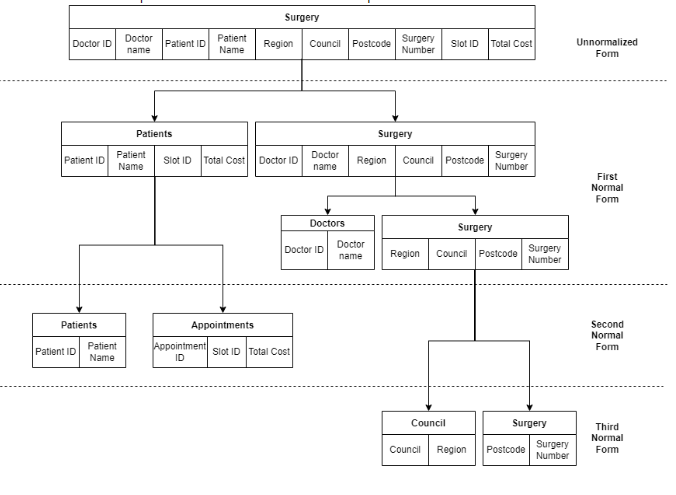
\includegraphics[width=0.8\textwidth]{normalisas-nf1-sampai-nf3.png}
    \caption{Proses Normalisasi dari NF1 sampai NF3}
\end{figure}

\end{document}